%!TEX root = ../main.tex
\chapter{Introdução}

\section{Motivação e Objetivos}

A nossa audição é um dos nossos sentidos mais importantes. É ela que nos permite identificar sinais e padrões no nosso mundo. Desde os tempo antigos, utilizamos a nossa audição para identificar situações de ameaças iminentes, como o rugido um predador prestes a atacar ou a buzina de um carro em alta velocidade. É também através dela que desenvolvemos o nossos métodos de comunicação.

Diversas indústrias utilizam o som para criar um ambiente imersivo para o usuário. Esse som pode utilizado para criar ditar o tom das experiências dos usuários. As indústrias de entrenimento (filmes, músicas, games e etc), por exemplo, utilizam o som para criar experiências mais realistas e divertidas \cite{bridgett2007}. O uso de som em aplicações audiovisuais tornou-se comum na década de 1920 com a sua utilização no cinema \cite{haussen2008som}.

Com isso, surge o seguinte problema: como criar o som para ser utilizado nessas aplicações? Para criar boas experiências para os usuários, o som tem que ser coerente com a cena apresentada \cite{rocchesso2003sounding}: O timbre e intensidade têm que ser compatível com o objeto (e.g.: sons metálicos vindo de metais e não de objetos de madeira), o áudio deve estar sincronizado com a cena e etc .

Uma das primeiras técnicas, e também uma das mais utilizadas, pelas indústrias é chamada de Foley. Nessa técnica, o artista de Foley utiliza elementos e objetos do mundo real para tentar sintezar as amostras de áudio de uma cena. O artista pode, por exemplo, utilizar pedaços de côcos para simular o som do trote de um cavalo \cite{bonebright2012were} ou folhas metálicas para simular o som de trovões (Ver \figref{fig:foley}).

\begin{figure}[ht]
	\centering
	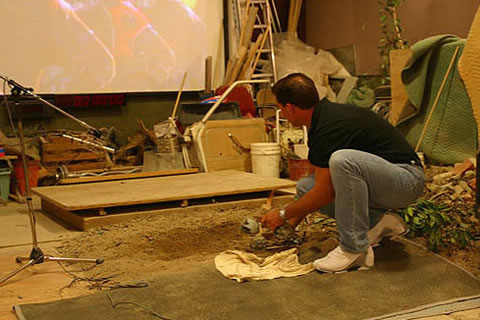
\includegraphics[width=0.6\textwidth]{introduction/foley.jpg}
	\caption[Artista de Foley em um estúdio de produção]{Artista de Foley em um estúdio de produção\footnotemark}\label{fig:foley}
\end{figure}

\footnotetext{Fonte: \url{http://www.t.sonypicturesstudiostours.com/uploads/img/std_content/soundeffects_05.jpg}. Acessado em 3 de Julho de 2016.}

Essa técnica, porém, tem várias limitações. Para garantir a qualidade da experiência sonora, os artista de Foley deve calibrar cuidadosamente para garantir a coerência do timbre e também para garantir a sincroniza entre o áudio e o vídeo. Isso requer mão-de-obra especializada. Embora a qualidade final do áudio gerado pela técnica seja boa, o custo e o tempo de produção podem inviabilizar o uso dessa técnica. Em muitos casos também há limitações físicas envolvidas: Seria inviável, por exemplo, usar esse tipo de técnica para sintetizar amostras de áudio geradas por uma estrutura metálica de grandes dimensões ou por uma grande esfera de diamante.

Em ambientes dinâmicos, no entanto, as limitações são ainda mais aparentes. No caso de uma aplicação virtual com interação de um usuário (um jogo, por exemplo), as interações que criariam o som seriam provenientes de comandos dados pelo usuário em tempo de execução. Nesse tipo de aplicação não é possível criar amostras sonoras durante a sua execução e também não é possível prever todas as possíveis interações do usuário.

Esse tipo de técnica não permite que o som dos objetos seja alterado de acordo com o estado da simulação em tempo de execução. O som gerado por um prato ao cair no chão, por exemplo, varia drasticamente de acordo com a posição de contato.  O uso de amostras sonoras nesse tipo de aplicação cria um ambiente acústico repetitivo que não se adapta à realidade do mundo virtual, o que desconstrói a imersão do usuário \cite{anderson1997sound}.

Recentemente, um novo tipo de técnica tem surgido: A Síntese de Som por Modelagem Física. Essa nova abordagem tenta sintetizar o som de uma cena através de simulações físicas. Esse tipo de abordagem em tese cumpre automaticamente os requisitos para criar uma boa experiência, pois o timbre, a intensidade seriam calculados de acordo com as propriedades físicas dos objetos e a sincronização surgiria naturalmente por conta da simulação. Esse tipo de técnica também poderia ser utilizado em aplicações dinâmicas, pois o som seria gerado em tempo de execução.

As técnicas de síntese por modelagem física costumam ser computacionalmente caras. Elas normalmente exigem que a solução de equações diferenciais complexas sejam calculadas em um domínio extenso. Acreditamos que este tipo de processamento possa ser eficientemente mapeado em arquiteturas de GPUs (Graphic Processing Units)\footnote{ GPUs são unidades de processamento especializadas, desenvolvidas para realizar cálculos em paralelo.}. Isso nos permitiria diminuir o tempo necessário para sintetizar o som de uma cena.

Por tais razões, o objetivo desse trabalho é desenvolver uma técnica de Síntese de Som por Modelagem Física e acelerá-la utilizando GPU.

\section{Estrutura do Trabalho}

Esse trabalho está estruturado da seguinte maneira: No Capítulo 2 descrevemos os conceitos matemáticos utilizados no estado-da-arte, o que inclui conceitos de Acústica e de Vibrações. No Capítulo 3 descrevemos os trabalhos relacionados, apresentando a evolução da área e discutindo as diferençãs entre Métodos por Modelagem Física e Métodos por Amostragem. No Capítulo 4 nós apresentamos o nosso método e também os detalhes de implementação. No Capítulo 5 nós descrevemos os experimentos utilizados para avaliar o desempenho do nosso método e também discutimos os resultados obtidos. Finalmente, concluímos esse trabalho no Capítulo 6 apresentando também planos para trabalhos futuros.
